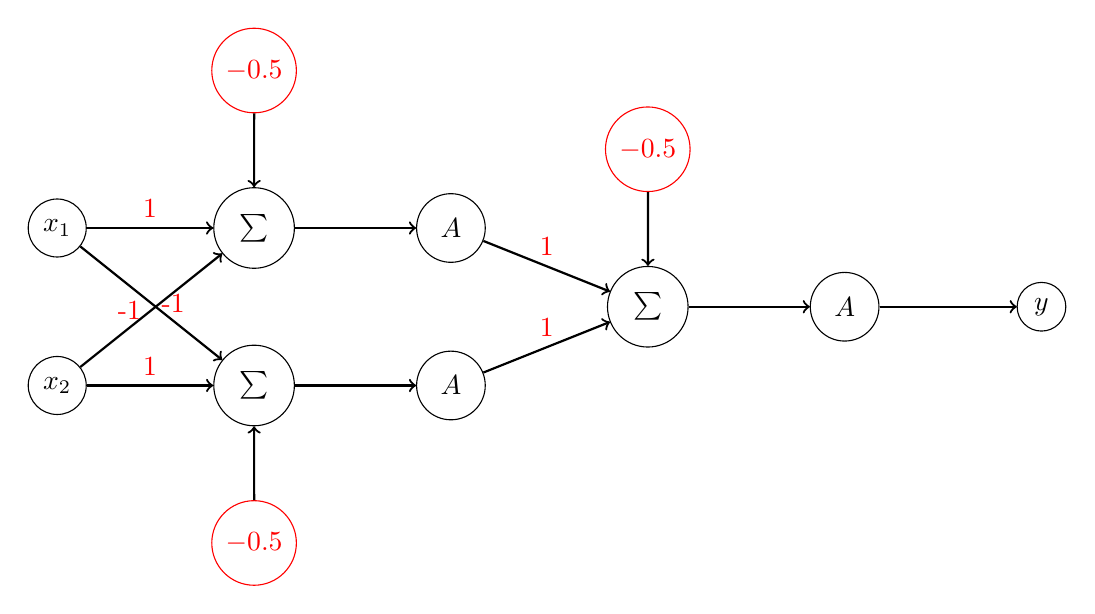
\begin{tikzpicture}[xscale = 2.5, yscale = 2]
  \node[draw, circle] (X1) at (0, 0){
    $x_{1}$
  };

  \node[draw, circle] (X2) at (0, -1){
    $x_{2}$
  };

  \node[draw, circle] (sum1) at (1, 0){
    \scalebox{1}{
      $\sum$
    }
  };

  \node[draw, circle] (act1) at (2, 0){
    \scalebox{1}{
      $A$
    }
  };

  \node[draw, circle] (sum2) at (1, -1){
    \scalebox{1}{
      $\sum$
    }
  };

  \node[draw, circle] (act2) at (2, -1){
    \scalebox{1}{
      $A$
    }
  };

  \node[draw, circle] (sum3) at (3, -0.5){
    \scalebox{1}{
      $\sum$
    }
  };

  \node[draw, circle] (act3) at (4, -0.5){
    \scalebox{1}{
      $A$
    }
  };

  \node[draw, circle, red] (bias1) at (1, 1){
    $-0.5$
  };

  \node[draw, circle, red] (bias2) at (1, -2){
    $-0.5$
  };

  \node[draw, circle, red] (bias3) at (3, 0.5){
    $-0.5$
  };

  \node[draw, circle] (y) at (5, -0.5) {
    $y$
  };

  \draw[thick, ->] (X1) -- node [above, red]{1} (sum1);
  \draw[thick, ->] (X1) -- node [below, right, red]{-1} (sum2);

  \draw[thick, ->] (X2) -- node [above, left, red]{-1} (sum1);
  \draw[thick, ->] (X2) -- node [above, red]{1} (sum2);

  \draw[thick, ->] (bias1) -- (sum1);
  \draw[thick, ->] (bias2) -- (sum2);
  \draw[thick, ->] (bias3) -- (sum3);

  \draw[thick, ->] (sum1) -- (act1);
  \draw[thick, ->] (act1) -- node[above, red]{1} (sum3);
  \draw[thick, ->] (sum2) -- (act2);
  \draw[thick, ->] (act2) -- node[above, red]{1} (sum3);
  \draw[thick, ->] (sum3) -- (act3);
  \draw[thick, ->] (act3) -- (y);
\end{tikzpicture}
